\NeedsTeXFormat{LaTeX2e}

\documentclass[12pt]{article}
\usepackage[letterpaper,portrait, margin=1in]{geometry}
\usepackage{booktabs, pgfplots, bm, multirow, amsmath, wrapfig, gensymb, graphicx}
\pgfplotsset{width=11cm,compat=1.9}
\renewcommand{\arraystretch}{1.5}
\usepackage[colorlinks=true, allcolors=blue]{hyperref}
\usepackage{indentfirst}
\usepackage{caption}



\begin{document}

%%%%%%%%%%%%%%%%%%%%%%%%%%%%%%%%%%%%%%%%%%%%%%%%%%%%%%%%%%%%
%%% COVER PAGE - TO BE COPIED AT BEGINNING OF LAB REPORT %%%
%%%      PLEASE ALSO FILL OUT WITH YOUR INFORMATION      %%%
%%%%%%%%%%%%%%%%%%%%%%%%%%%%%%%%%%%%%%%%%%%%%%%%%%%%%%%%%%%%

\begin{titlepage}

       %\vspace*{.5cm}
        \begin{center}
        \textbf{\huge PH-291 Physics Lab} \\ 
        \textbf{\Large Professor Corn-Agostini} \\ 
        \textbf{\Large Fall 2022} \\ 
        \vspace*{.5cm}  
        \textbf{\large Lab \# 3: Pinhole Photography}
        \vspace{0.5cm}
        \end{center}
       
\noindent Your Name: Perla Berkovitz\\ \\
\noindent Your Lab Section: E\\ \\
\noindent Your Lab Instructor: Professor Corn-Agostini\\ \\
\noindent Your Lab Partner's Name: Sharon Sitt\\ \\
\noindent Read and sign Academic Integrity Statement:\\

\noindent {\em I hereby attest that I have not given or received any unauthorized assistance on this assignment.}

    \begin{center}
    \line(1,0){300} \\
    Sign here
    \end{center}

\noindent\textbf{\large Grading Rubric} \\ \\
\renewcommand{\arraystretch}{1.5}
%\large
\begin{tabular}{|l|c|r|l|} \hline
 {\bf SECTION } & {\bf POINTS} & {\bf GRADE}\\\hline 
Self Portrait & 9 & \\\hline
Demonstration of Physical Principle & 4 & \\\hline
Alternate Developer & 2 & \\\hline \hline 
{\em Total} & 15 & \\ \hline
\end{tabular}

\end{titlepage} 




\newpage
\section*{Selfie Improvement}
    \begin{minipage}{.5\textwidth}
      \centering
      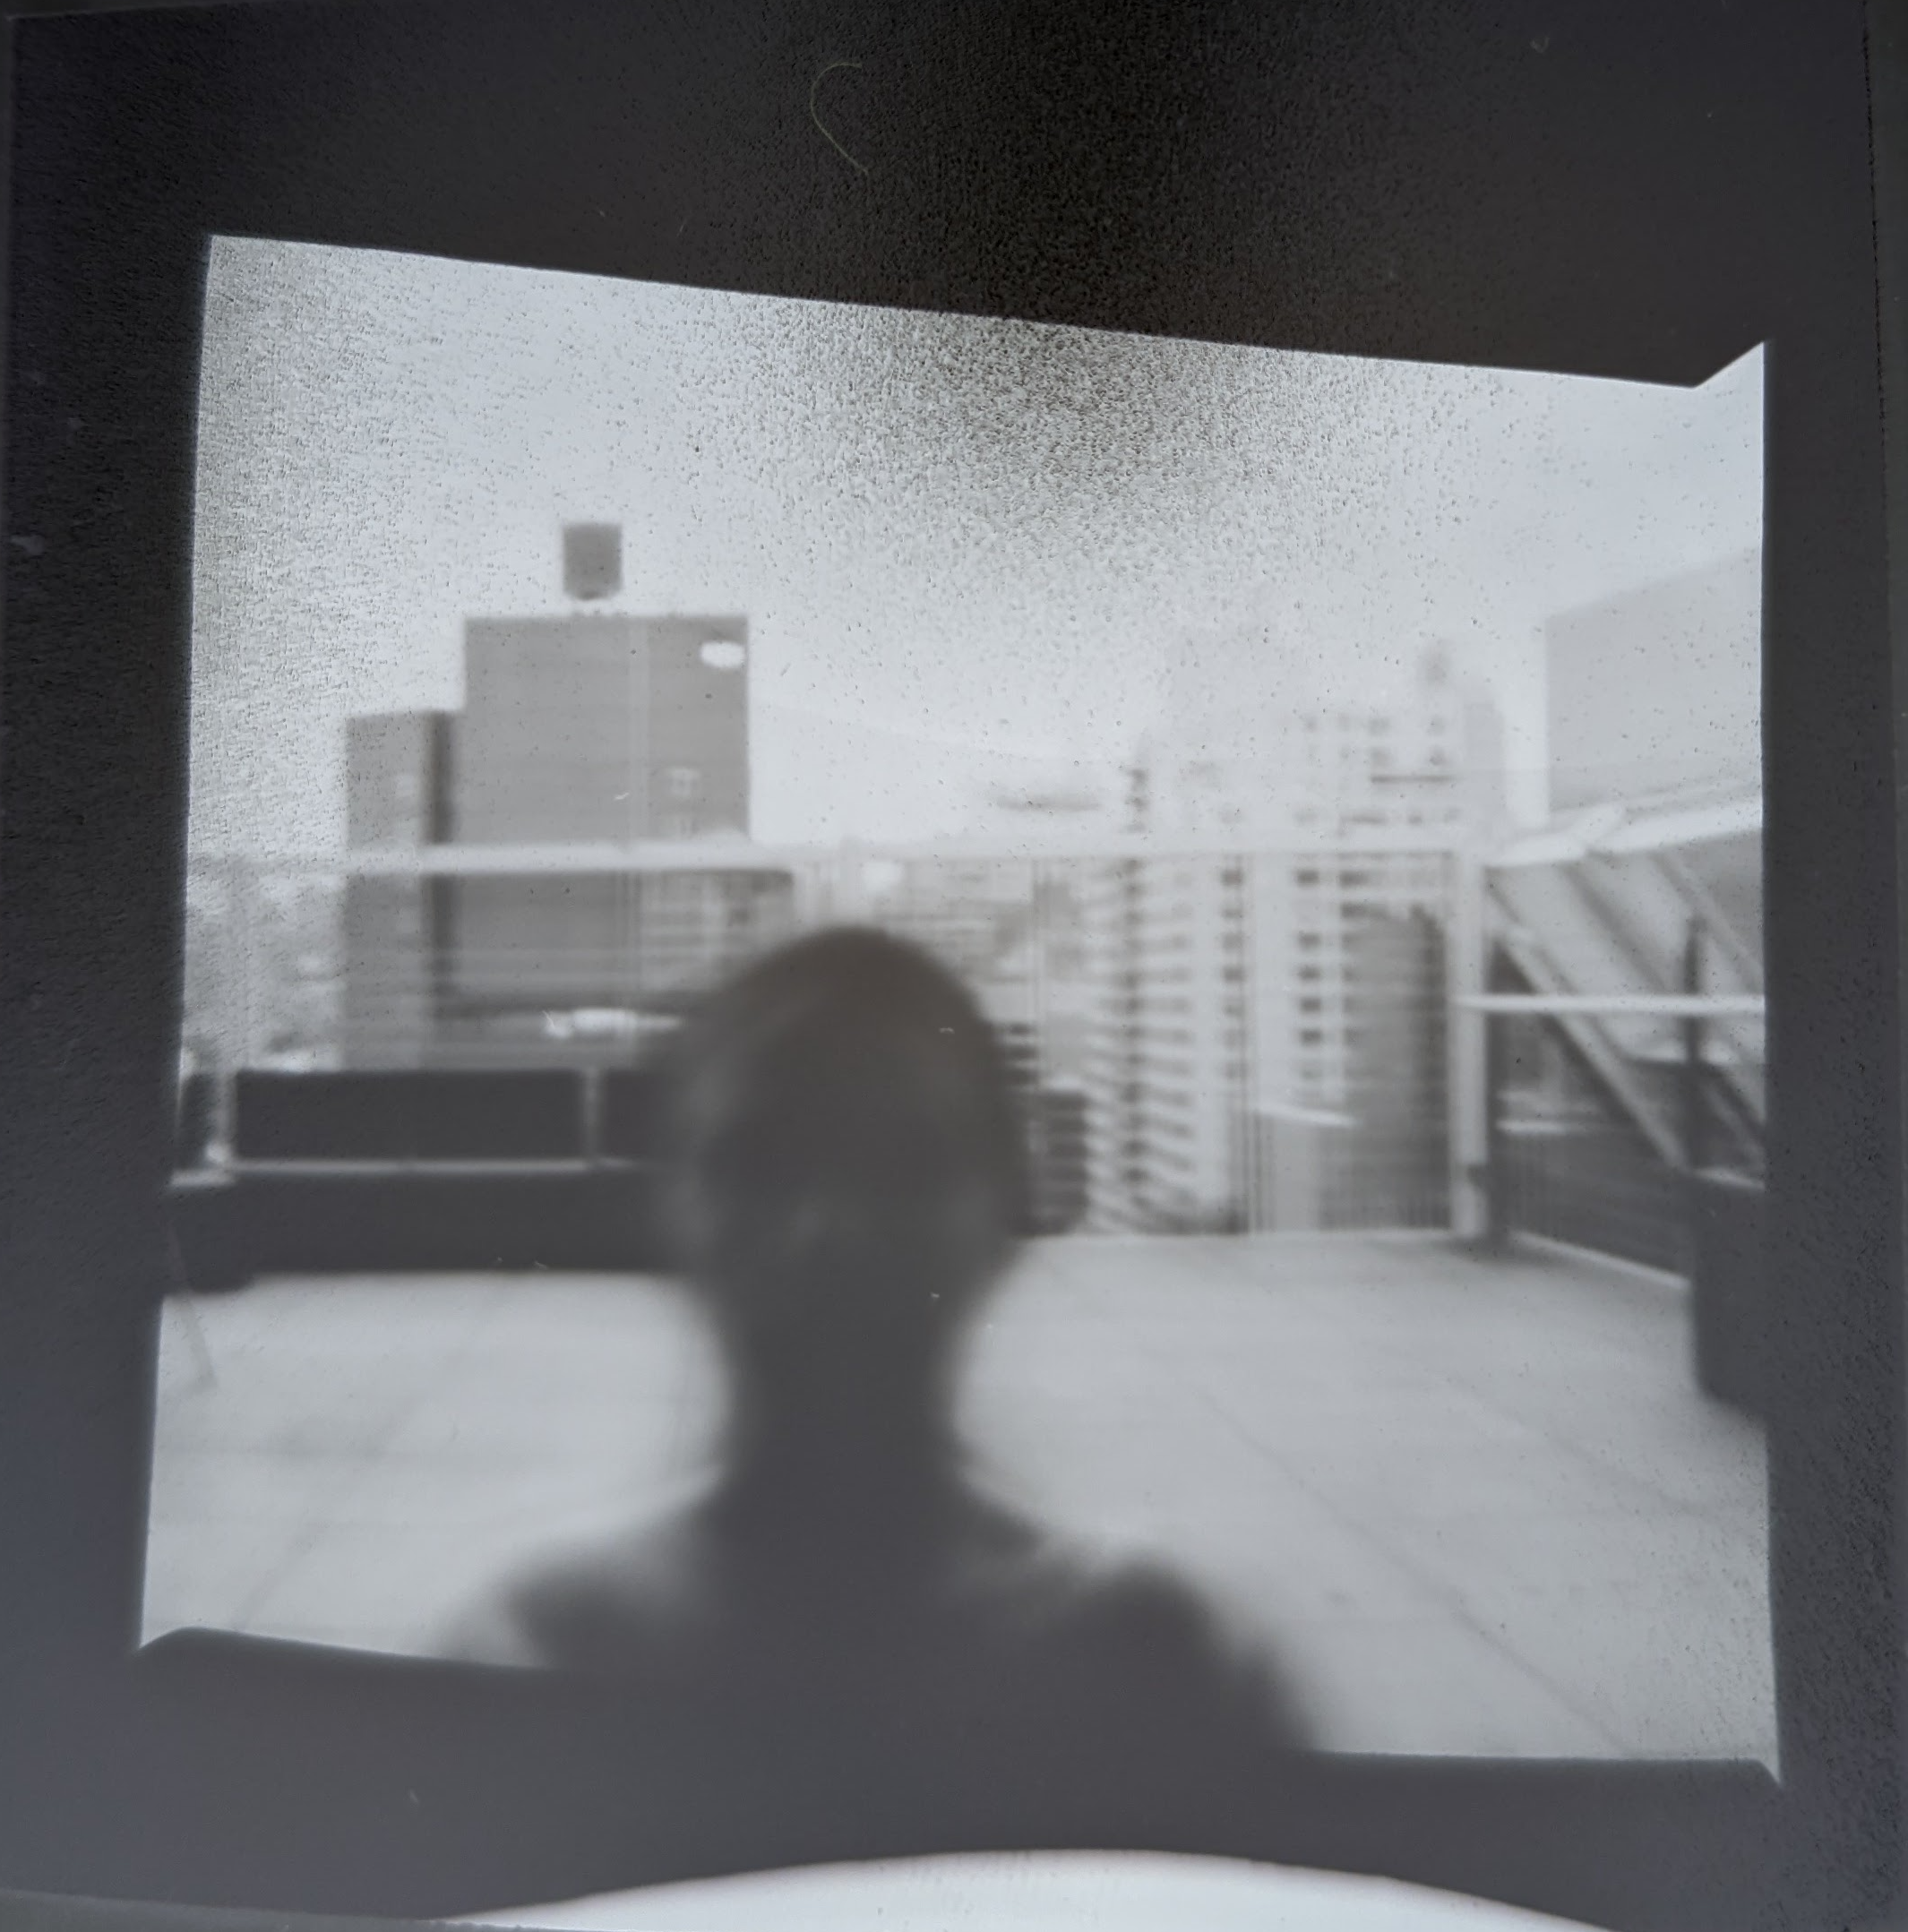
\includegraphics[width=\linewidth]{bad selfie.png}
      \captionof{figure}{First Selfie Taken}
      \label{fig:test1}
      \vspace{5mm}
    \end{minipage}%
    \begin{minipage}{.5\textwidth}
      \centering
      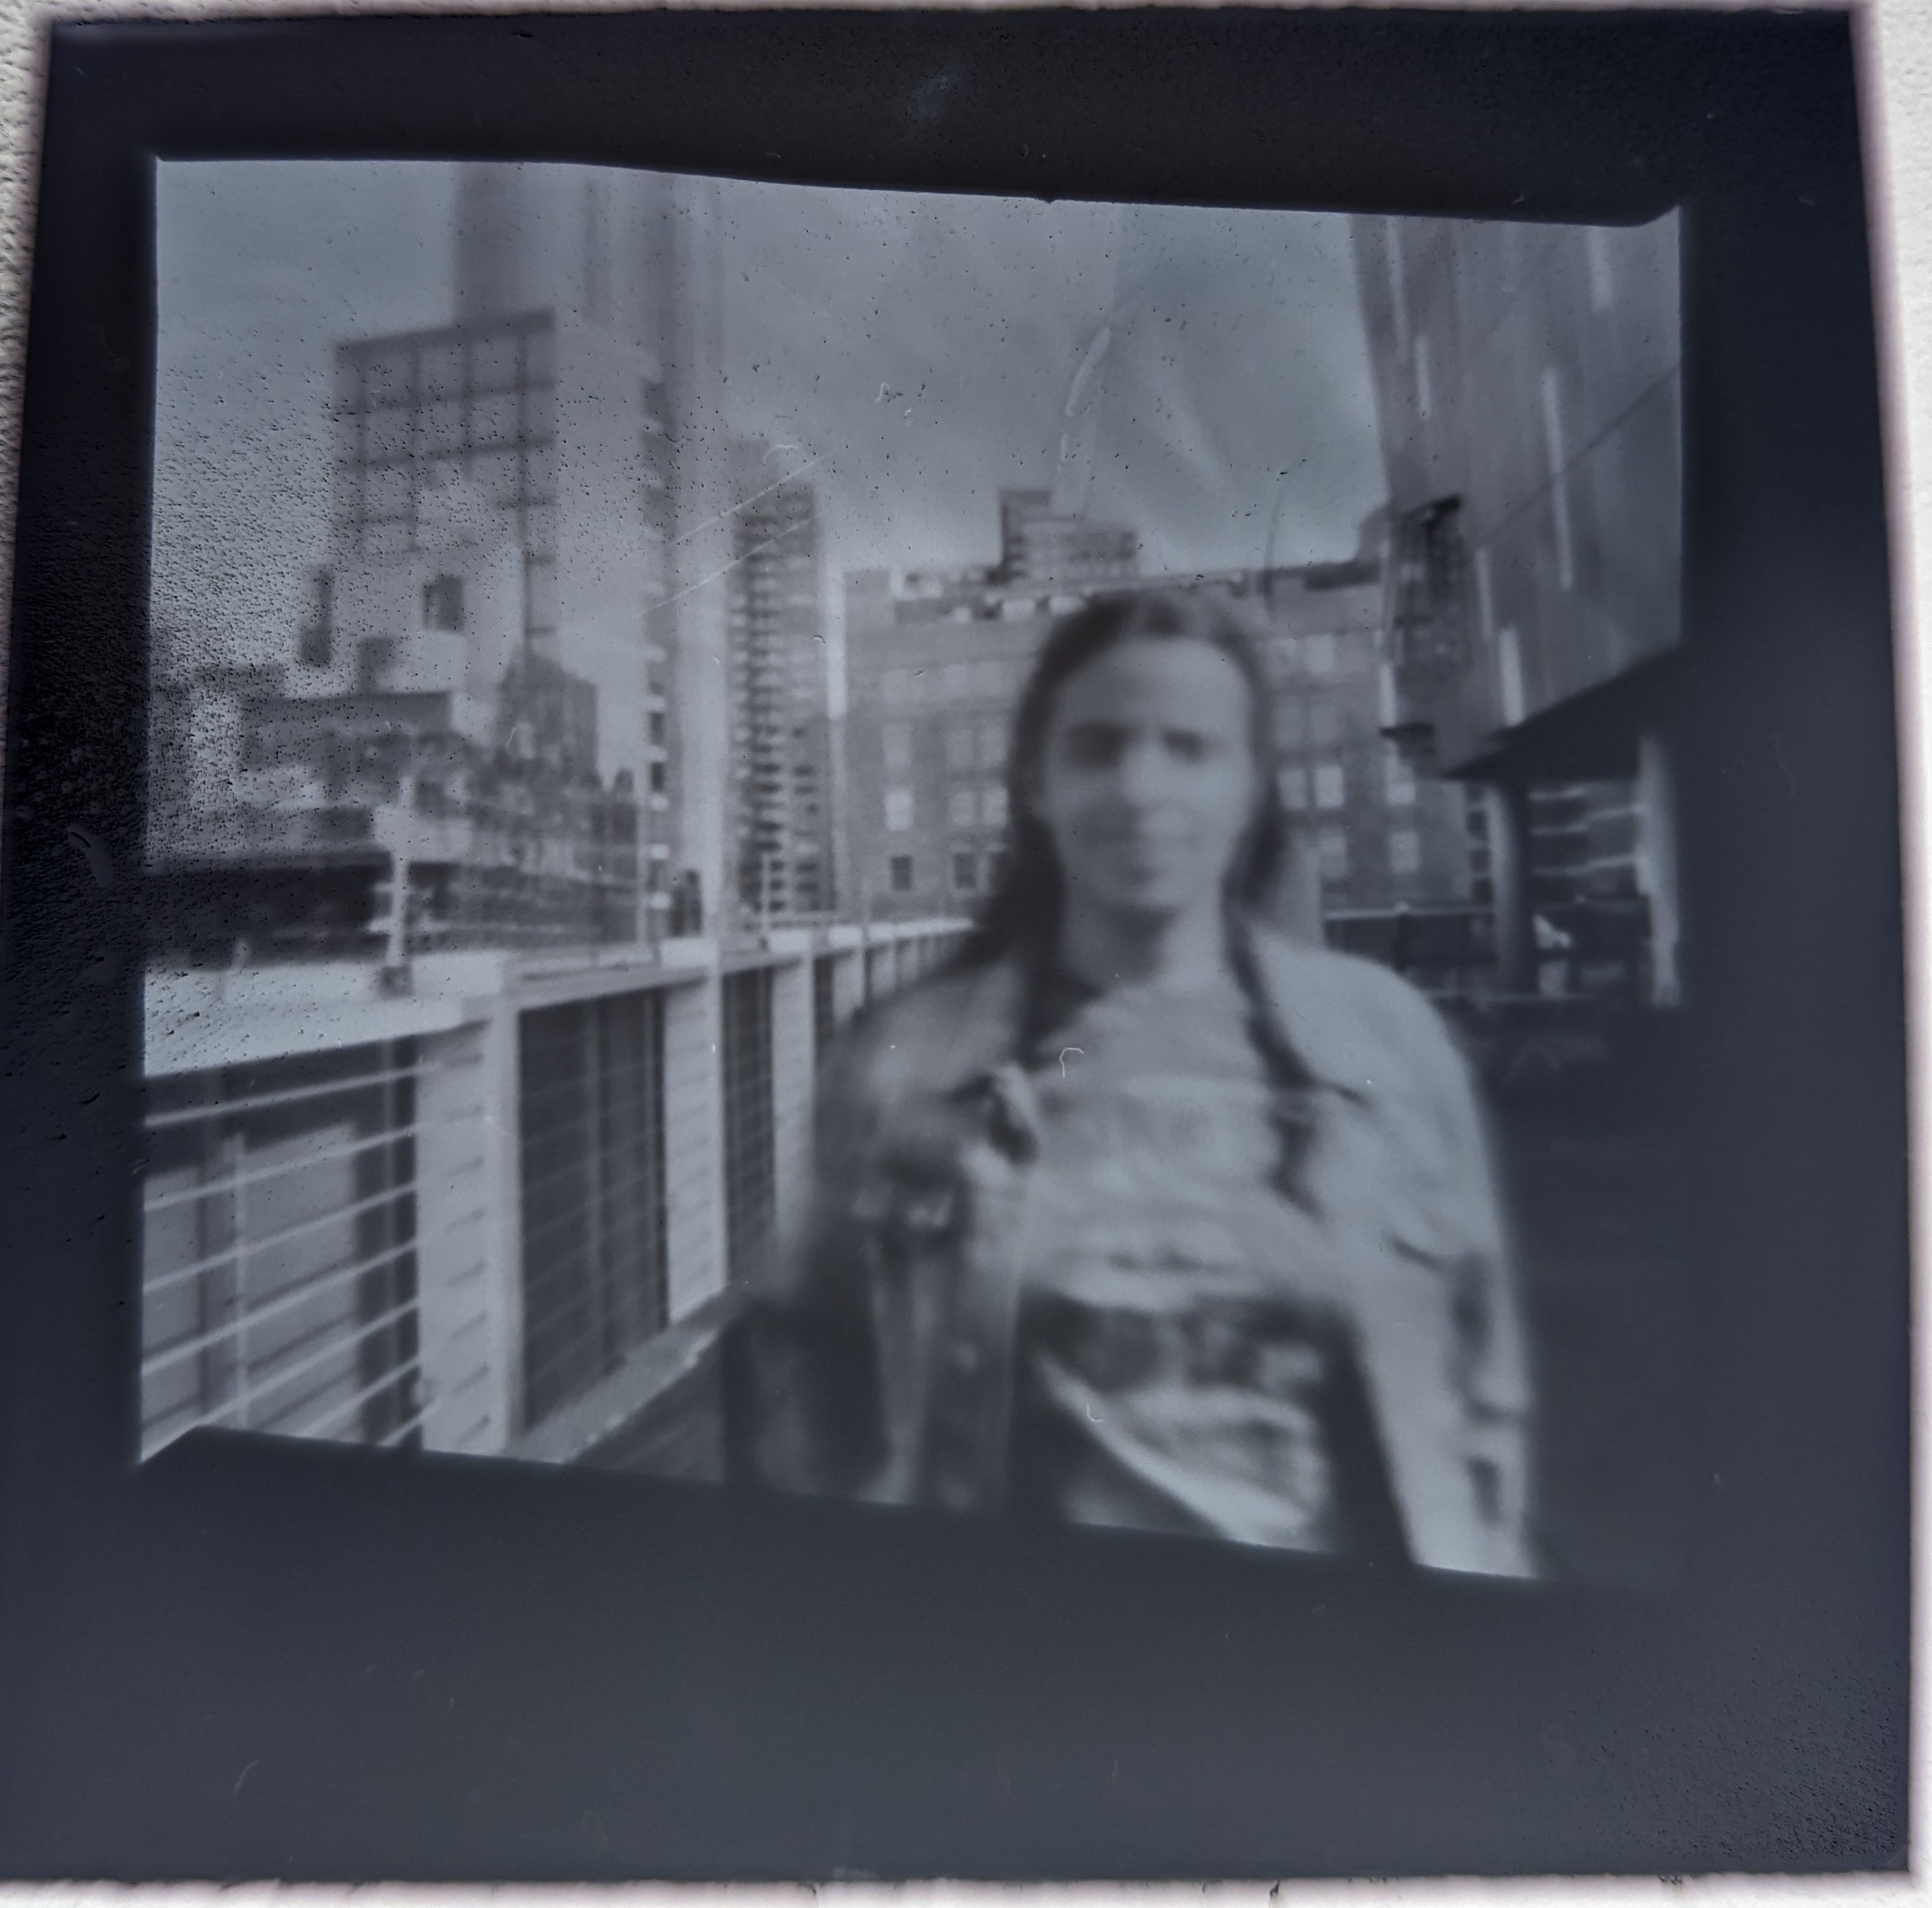
\includegraphics[width=\linewidth]{good selfie.png}
      \captionof{figure}{Improved Selfie}
      \label{fig:test2}
      \vspace{5mm}
    \end{minipage}
    
    When the first selfie was taken, I had positioned myself with the light behind me. This caused the camera to not have enough light on my face to capture a detailed image. In the improved selfie, there was better lighting, which allowed for a better image to be captured.
\section*{Physical Phenomenon}
\begin{center}
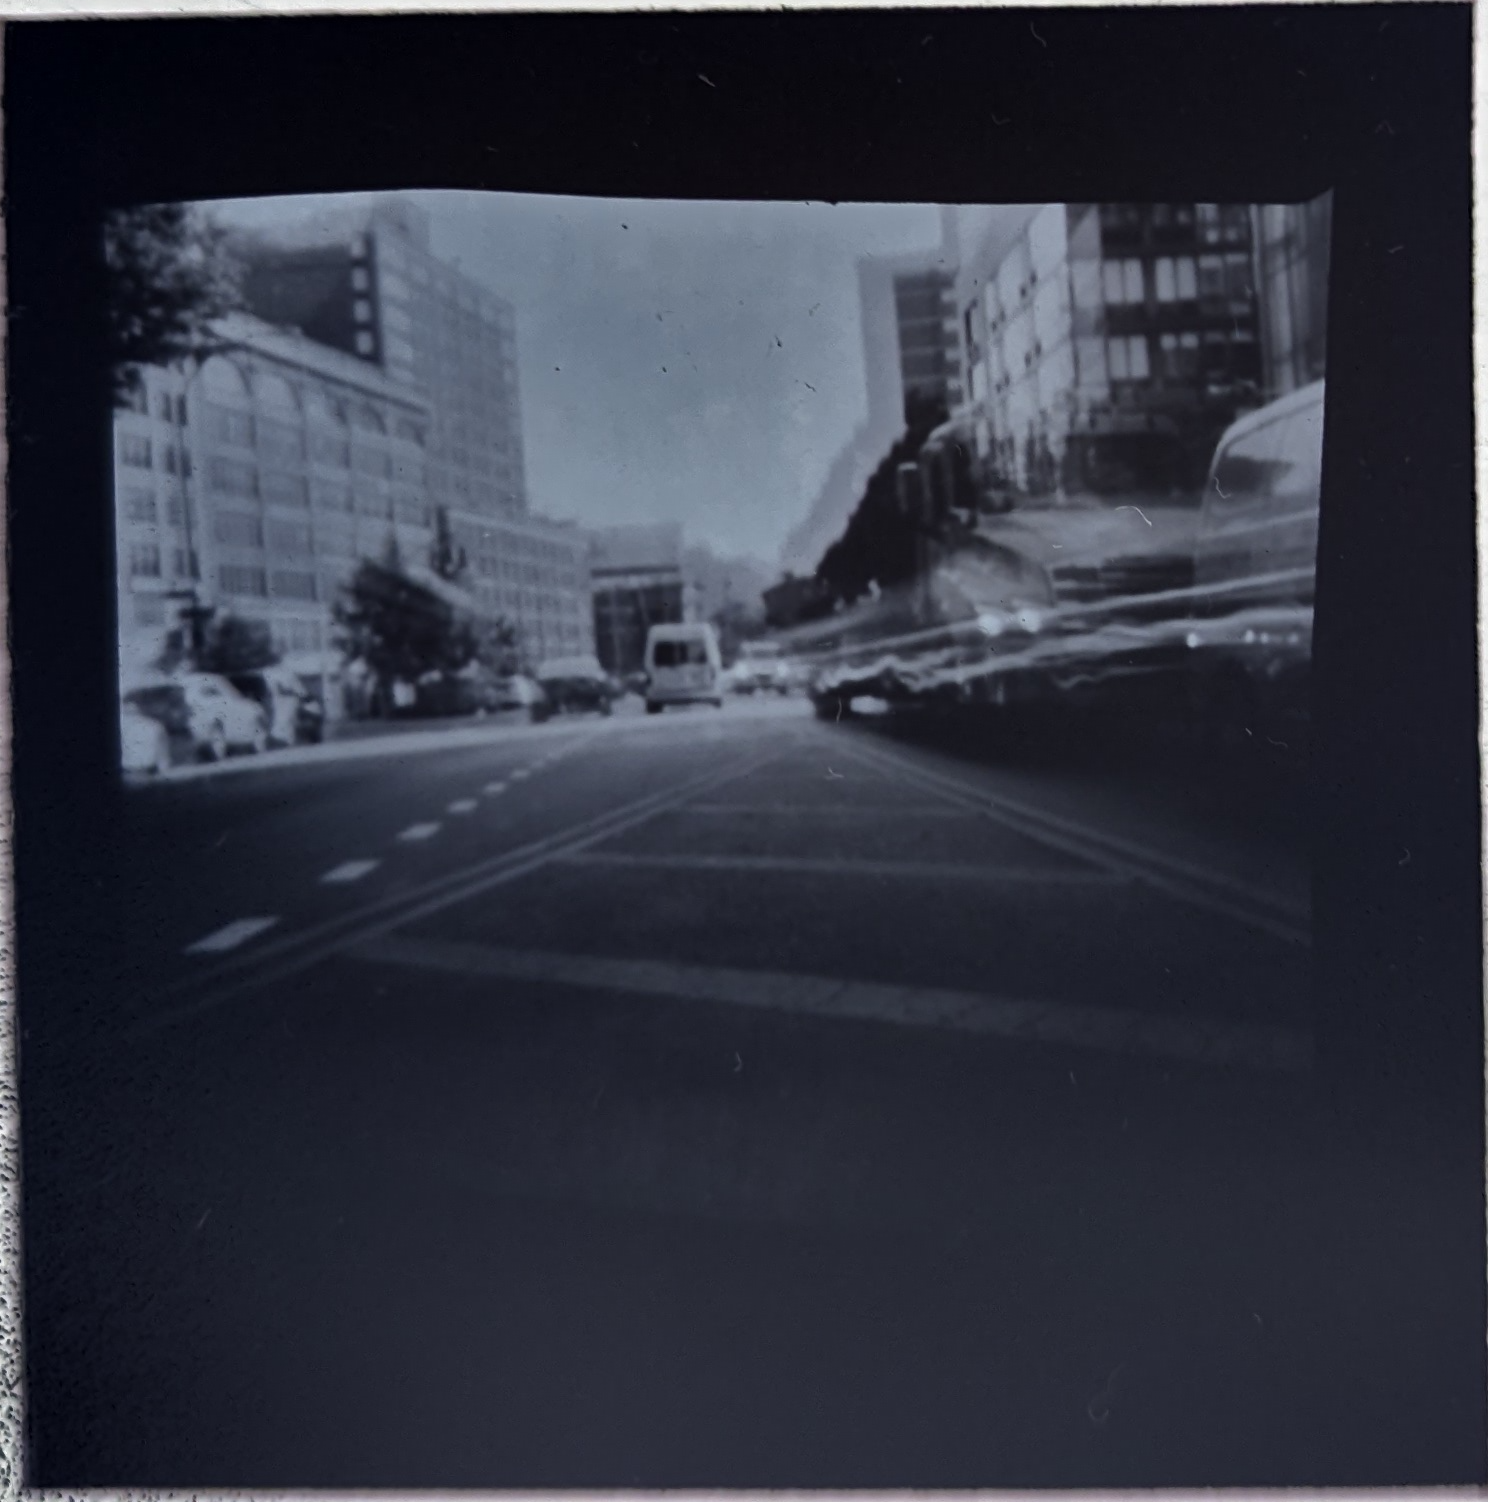
\includegraphics[scale=0.2]{physical principle.png}
\captionof{figure}{Physical Phenomenon}
\end{center}
  For my physical phenomenon, I chose motion and relative velocity. In the image, the motion streaks on the right hand side are a result of the cars traveling past at some velocity, while the camera remained stationary. Like the camera, other cars in the image and the surroundings remain stationary which have velocity = 0.
\section*{Alternative Developer Recipe}
\begin{center}
    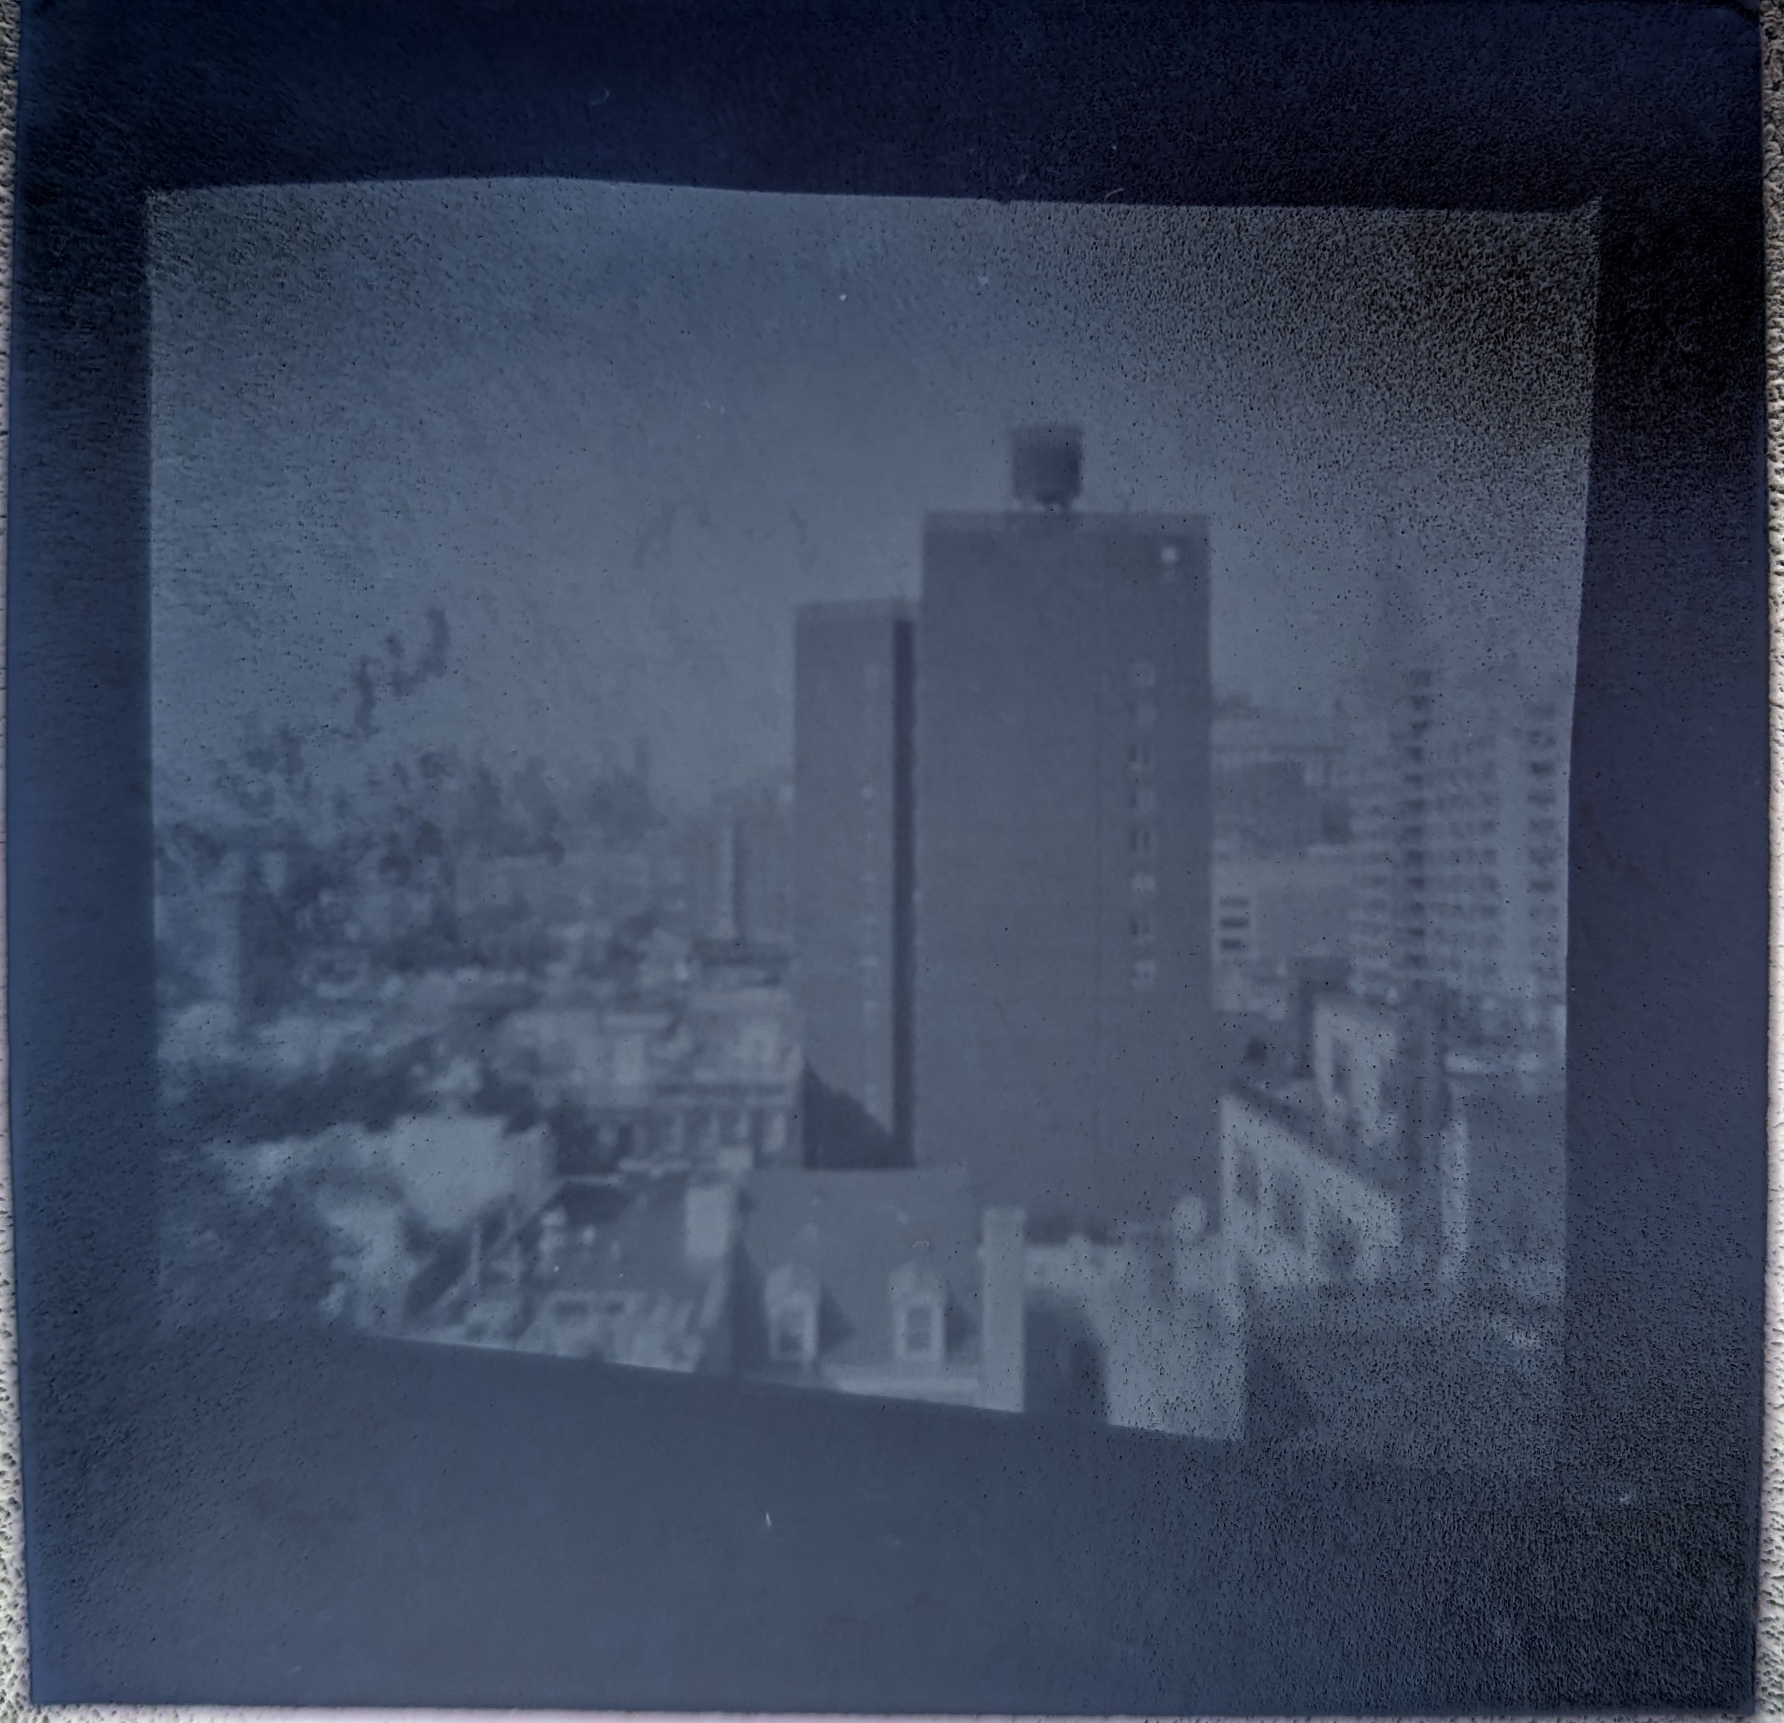
\includegraphics[scale=0.2]{alternate developer.png}
    \captionof{figure}{Alternate Developer}
    \end{center}
\noindent200 mL Water\\
1 g Vitamin C\\
1.2 g Instant Coffee\\
10 g Washing Soda\\
\end{document}